\documentclass[aspectratio=169]{beamer}

\usepackage{blindtext}

\usetheme{Janelia}

\usepackage{people}
\usepackage[english]{babel}
\usepackage[T1]{fontenc}

\usepackage[overlay,absolute]{textpos}

\usepackage{tabularx}
\usepackage{booktabs}
%\usepackage{enumitem}

\usepackage{textcomp}
\usepackage{ragged2e}
\usepackage{gensymb,marvosym}

\usepackage{helvet,eurosym}

\usepackage{multimedia}
\usepackage{calc}
\usepackage{siunitx}

\usepackage{tikz}
\usetikzlibrary{arrows,backgrounds,patterns}
% TikZ gray color model is wrong, particularly for shading!
\definecolor{litelitegray}{rgb}{0.85,0.85,0.85}
\definecolor{gray}{rgb}{0.5,0.5,0.5}
\definecolor{black}{rgb}{0,0,0}
\definecolor{white}{rgb}{1,1,1}
\definecolor{darkgreen}{rgb}{0,0.75,0}
\definecolor{darkred}{rgb}{0.75,0,0}
\definecolor{darkmagenta}{rgb}{0.75,0,0.75}
\definecolor{darkblue}{rgb}{0,0,0.75}
\definecolor{mycyan}{rgb}{0.0,0.9,0.9}

\tikzstyle{task}=[rectangle, rounded corners=4pt, draw=black, fill=blue!20, thick, inner sep=8pt, minimum size=1.25cm, text width=2.5cm, text centered]
\tikzstyle{pre}=[<-, shorten <=2pt,>=stealth',thick]
\tikzstyle{post}=[->,shorten >=2pt,>=stealth',thick]
\tikzstyle{text}=[anchor=base,inner sep=0pt]


\usepackage{pdfpages}

\usepackage{algorithm}
\usepackage{algpseudocode}

\newcommand{\inout}[2]{%
	\begin{tabbing}
		\textbf{Output:~}\= output \kill
		\textbf{Input:}\> #1 \\
		\textbf{Output:}\> #2
	\end{tabbing}%
}
\newcommand{\proc}[1]{%
	\textbf{#1}%
}
\newcommand{\callproc}[2]{%
	\proc{#1}(#2)%
}
\newcommand{\var}[1]{%
	\mathit{#1}%
}
\newcommand{\vect}[1]{%
	\mathbf{#1}%
}

\newcommand{\greenTxt}[1]{%
    \color{HHMIGreenB} #1%
}

\newcommand{\backupbegin}{
  \newcounter{finalframe}
  \setcounter{finalframe}{\value{framenumber}}
}

\newcommand{\backupend}{
  \setcounter{framenumber}{\value{finalframe}}
}

\newcommand{\code}[1]{\texttt{#1}}



\newlength\imagesep
\setlength\imagesep{0.125cm}
\setlength\parskip{0pt}
\newlength\lwidth
\newlength\stepwidth
\newlength\tilesize%
\newlength\colsep%
\newlength\colwidth%
\newlength\templen%
\newlength\imgscale%

%\renewcommand\Vec[1]{\ensuremath{\vec{#1}}}
\newcommand\Mat[1]{\ensuremath{\mathbf{#1}}}
\newcommand\trnsp{\ensuremath{\mathsf{T}}}
%\newcommand\unit[1]{\ensuremath{\mathrm{#1}}}
\newcommand\Dom{\ensuremath{\Omega}}
\newcommand\Codom{\ensuremath{\mathbb{T}}}

\DeclareMathOperator \norm {norm}
\DeclareMathOperator \abs {abs}
\DeclareMathOperator \Tr {tr}
\DeclareMathOperator \Det {det}

\newcommand{\rhoa}[1]{\rho_{#1}}
\newcommand{\rhofit}[1]{\rhoa{\text{fit}#1}}
\DeclareMathOperator*{\argmin}{arg\,min}
\newcommand{\mtilde}{\widetilde{m}}
\newcommand{\stilde}{\tilde{s}}
\newcommand{\rtilde}{\tilde\rho{}}
\newcommand{\window}[2]{w(#1,#2)}
\newcommand{\zref}{z_{\text{ref}}}
\newcommand{\rhom}{\Mat{S}}
\newcommand\RangedWindow[2]{w_{#1}(#2)}
\newcommand\RRangedWindow[1]{\RangedWindow{r}{#1}}
\newcommand{\rhomTransformed}{\mathcal{S}}
\newcommand{\oneOverDiffWeight}[2]{\frac{1}{1+|#1-#2|}}
\newcommand{\bellCurveWeight}[2]{e^{\left(\frac{#1-#2}{2\sigma}\right)^2}}
\newcommand{\fitWindowWeight}{\window{z}{\zref}}
\newcommand{\shiftOpinionWeight}{\window{z}{\zref}}

\newcommand\ie{i.\,e.\@\xspace}
\newcommand\Ie{I.\,e.\@\xspace}
\newcommand\eg{e.\,g.\@\xspace}
\newcommand\Eg{E.\,g.\@\xspace}
\newcommand\etc{\emph{etc}.\@\xspace}

\newcommand\citefoot[1]{
    \begin{textblock}{12}(6.5,15)
        %{\color{HHMIGrayB} \tiny Zhang et al.~ 2018. PMID 30033368 }
        %{\color{HHMIGreenB} \tiny Zhang et al.~ 2018. PMID 30033368 }
        {\color{HHMIGrayB} \tiny #1}
    \end{textblock}
}

\newcommand\leftfoot[1]{
    \begin{textblock}{12}(0.5,13.7)
        {\color{gray} \scriptsize #1}
    \end{textblock}
}

\newcommand\rightfoot[1]{
    \begin{textblock}{15}(0.5,13.7)
        {\color{gray} \scriptsize \hspace*{0pt}{\hfill} #1}
    \end{textblock}
}

\title[BigWarp]{\LARGE{Advanced registration of big image data} }
%\author{John Bogovic {\footnotesize \emph{(Saalfeld lab)}}}
\author{John Bogovic}

%\institute[HHMI Janelia]{HHMI Janelia Research Campus}
\date{12 Sept 2023}

\subject{Talks}

\tikzstyle{every picture}+=[remember picture]

\begin{document}

\setbeamercolor{normal text}{bg=white}
\setbeamercolor{normal text}{bg=black,fg=white}
\usebeamercolor[fg]{normal text}

\begin{frame}[plain]
  \titlepage
\end{frame}

\setbeamercolor{normal text}{bg=white,fg=black}
\usebeamercolor[fg]{normal text}

\begin{frame}{Outline}
  Image Registration
  \vspace{1.0em}
  \begin{itemize}
      \setlength\itemsep{1.0em}
      \item Transformations
      \item Image Geometry
      \item Practical algorithmic details
      \begin{itemize}
          \setlength\itemsep{0.5em}
          \item a
          \item b
          \item c
      \end{itemize}
  \end{itemize}
\end{frame}


\begin{frame}{Image registration}

    \vspace{0.2cm}
    \only<1>{
        \begin{center}
            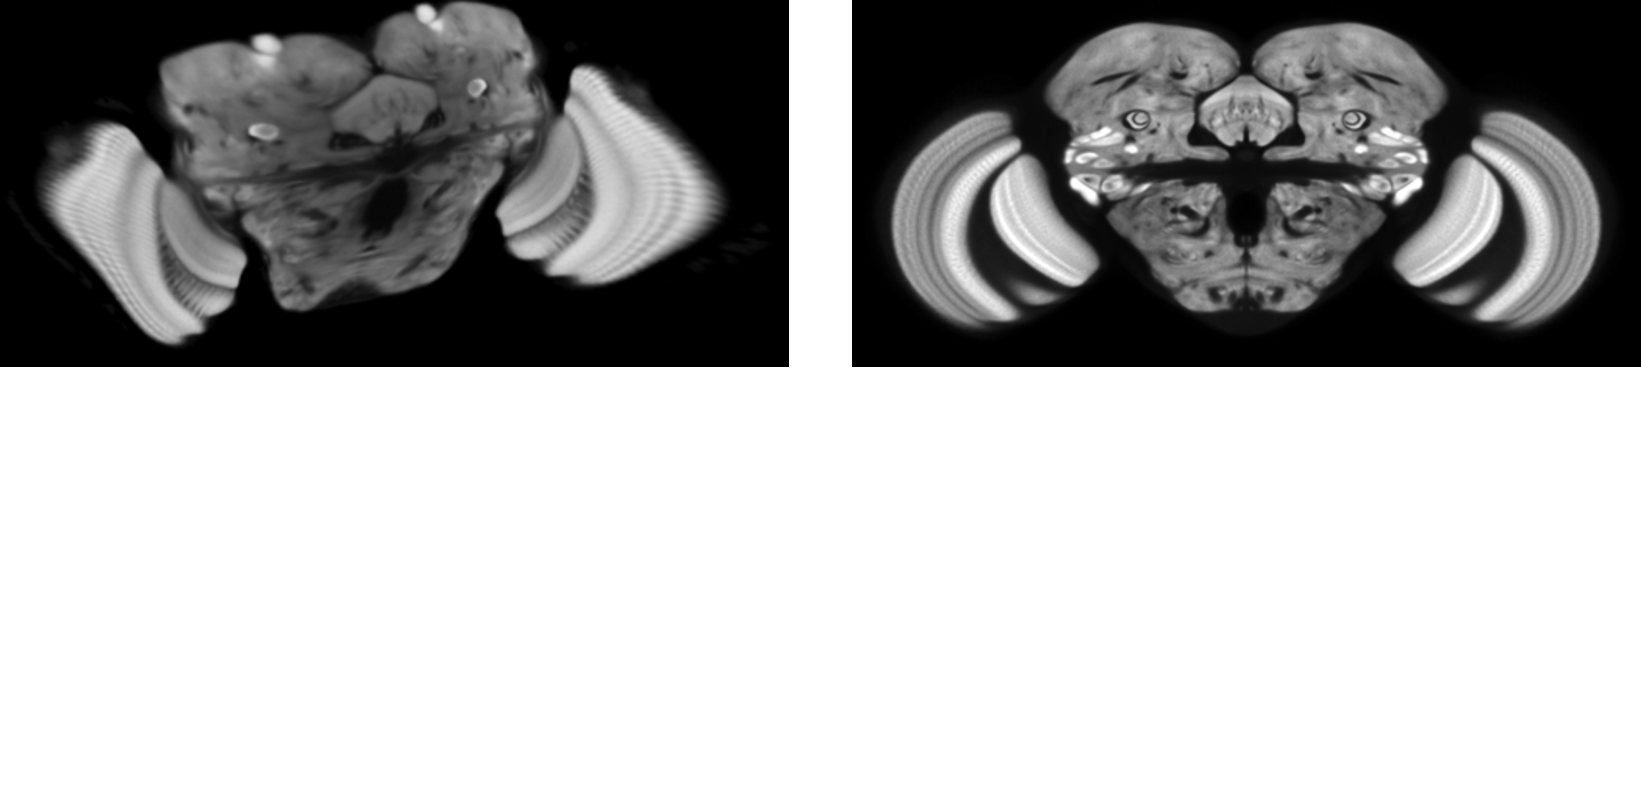
\includegraphics[width=0.8\paperwidth]{figures/imgRegFig_v2-1.pdf}
        \end{center}
    }
    \only<2>{
        \begin{center}
            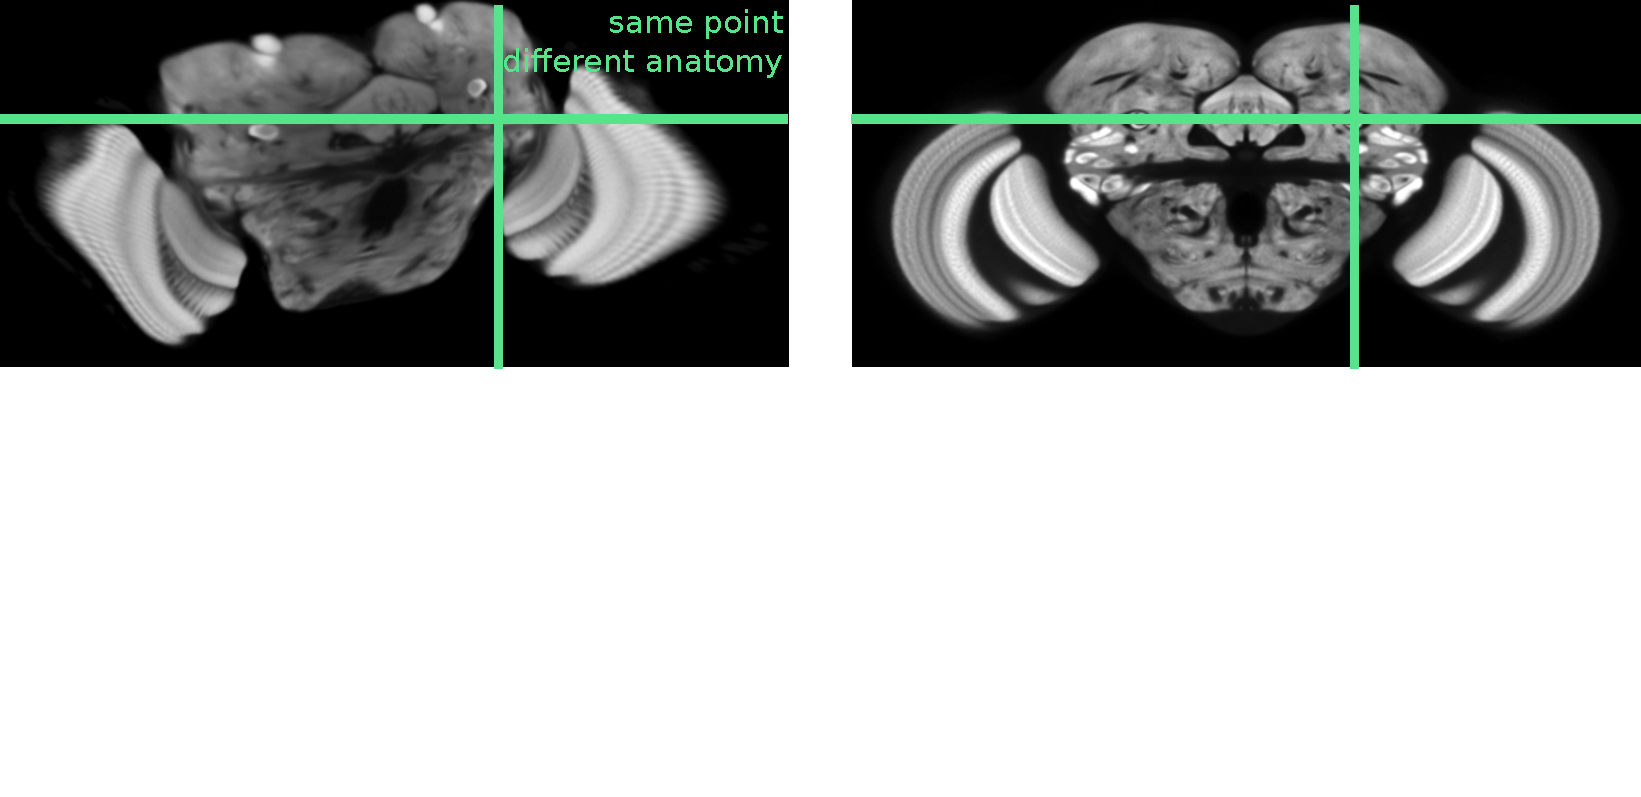
\includegraphics[width=0.8\paperwidth]{figures/imgRegFig_v2-2.pdf}
        \end{center}
    }
    \only<3>{
        \begin{center}
            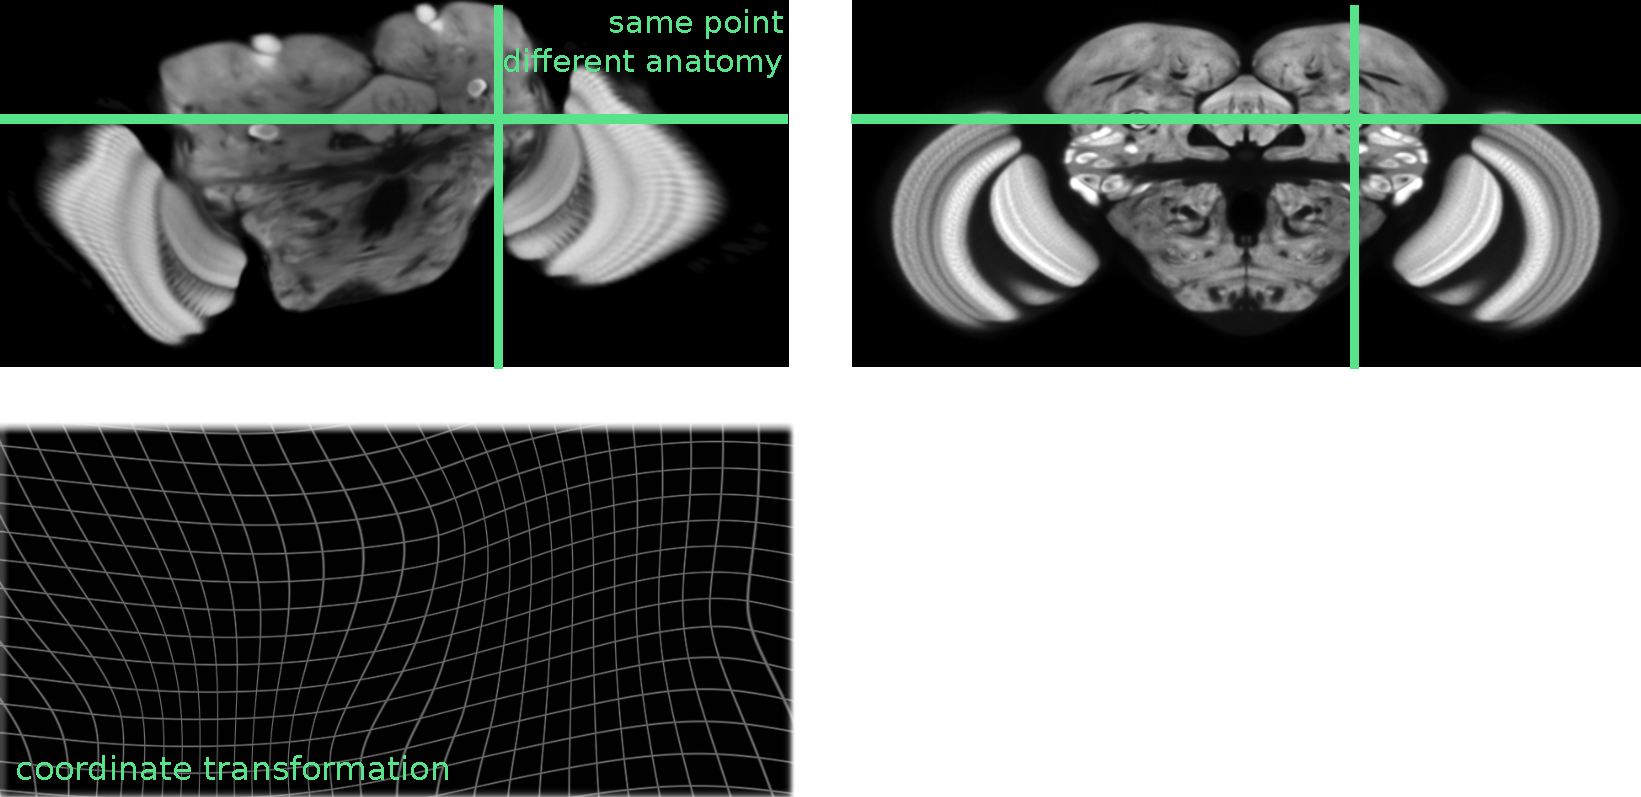
\includegraphics[width=0.8\paperwidth]{figures/imgRegFig_v2-3.pdf}
        \end{center}
    }
    \only<4>{
        \begin{center}
            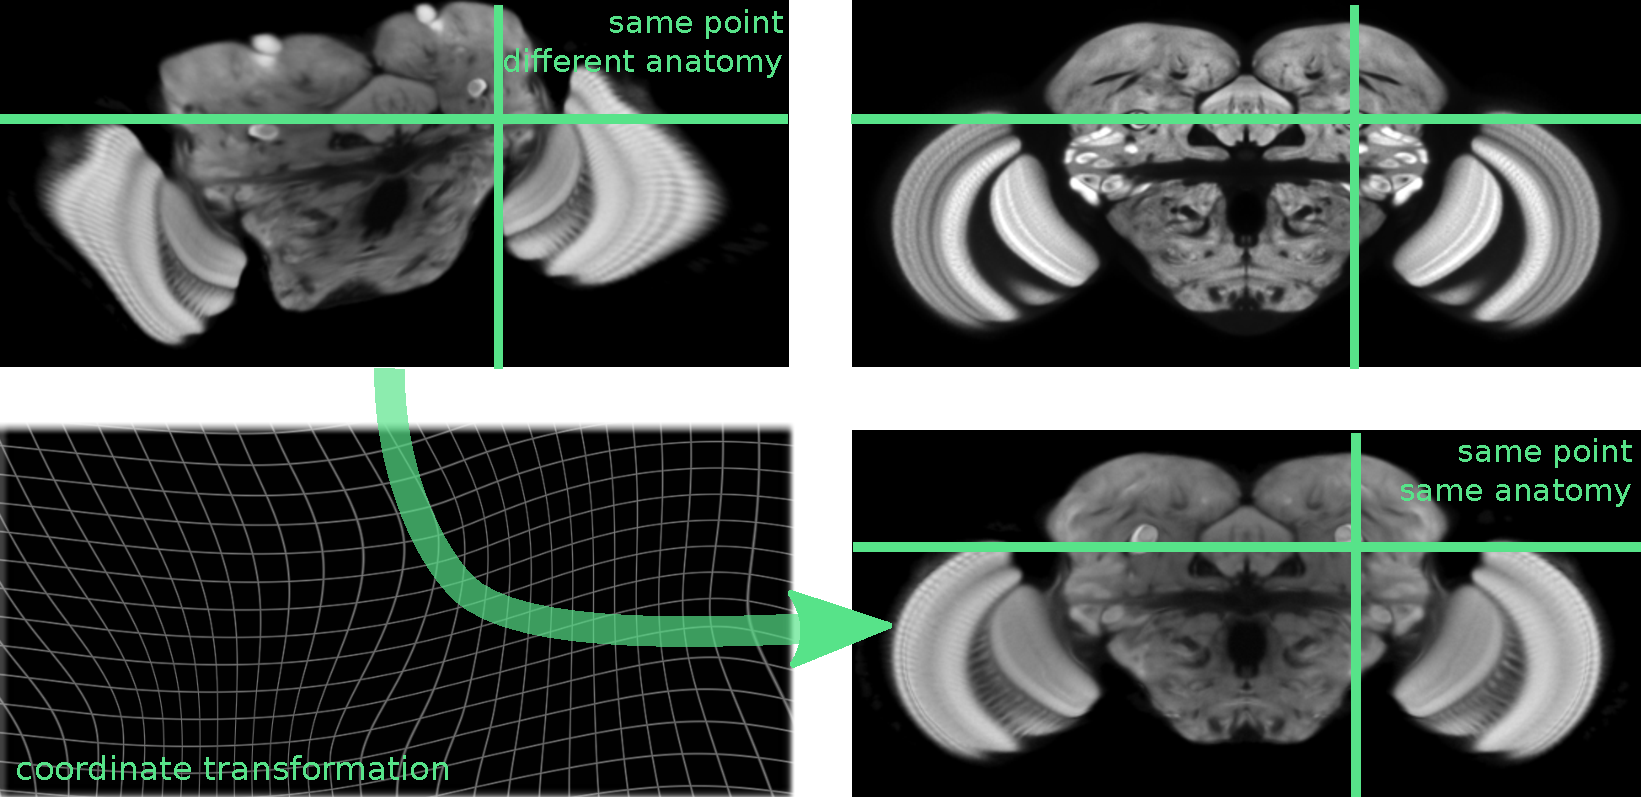
\includegraphics[width=0.8\paperwidth]{figures/imgRegFig_v2-4.pdf}
        \end{center}
    }

\end{frame}

\begin{frame}{Key idea}

    The primary output of an image registration algorithm is \\
    the \emph{transformation}. \\ 
    \vspace{1em}
    A secondary output of an image registration algorithm is \\ 
    the \emph{transformed moving image}.

\end{frame}

\begin{frame}{What is a transformation}

    %\only<1>{
    %        \vspace{1em}  
    %        \includegraphics[height=0.7\paperheight]{figures/transforms/TransformsCoordinateSystem-1.pdf}
    %}
    %\only<2>{
            \vspace{1em}  
            \includegraphics[height=0.7\paperheight]{figures/transforms/TransformsCoordinateSystem-2.pdf}


        \begin{textblock}{7}(8,6.0)
            Transformations are functions that: \\
            take points (coordinates) as inputs \\
            produce points (coordinates) as outputs.
        \end{textblock}
    %}

\end{frame}


\begin{frame}{Image geometry}
    \begin{center}
        \includegraphics[width=0.8\paperwidth]{figures/ImageOriginAndSpacing.pdf}
    \end{center}
    \citefoot{image from ITK Software Guide}
\end{frame}


\begin{frame}{Many relationships are transformations}

    \vspace{0.7em}
    \begin{center}
      \includegraphics[width=0.7\paperwidth]{figures/transforms/transformsSlide.pdf}
    \end{center}

    \vspace{-0.4em}Join the conversation at \code{github.com/ome/ngff}

\end{frame}


%\begin{frame}{Transformations in OME-Zarr}
%
%    \begin{center}
%        Efficient data access puts the ``big'' in BigWarp \\
%        \vspace{1em}Chunked file formats* makes array access efficient \\
%        \vspace{1em}Ome-Zarr standardizes critical metadata
%    \end{center}
%
%    \rightfoot{ \scriptsize{ *HDF5, N5, Zarr, etc.}}
%
%\end{frame}


\begin{frame}{Key ideas}

    Pixels (entries in the image array) are \emph{point samples}. \\
    \vspace{1em}
    Pixels are located in \emph{physical coordinates} \\
    \vspace{2em}
    Reinforce these ideas in \code{ResampleImages.ipynb}

\end{frame}

\begin{frame}[plain]%
\frametitle{point and image transformations}
    
    Define:
    \begin{itemize}
        \item The \emph{forward} transformation maps \emph{points} from
            \newline moving to target space.
        \item The \emph{inverse} transformation maps \emph{points} from
            \newline target to moving space.
    \end{itemize}

    \only<2>{
    Then:
    \begin{itemize}
        \item We need the \emph{inverse} transformation to map
            \emph{images} from \newline moving to target space
        \item We need the \emph{forward} transformation to map
            \emph{images} from \newline target to moving space
    \end{itemize}

    The following will explain why this is the case.
    }

\end{frame}


\begin{frame}[plain]%
\frametitle{Transforms on a grid}

    \only<1>{
        \begin{textblock}{14}(1,12)
            We have a moving image that we want to transform, and render
            on a new, target image grid.
        \end{textblock}

        \begin{tikzpicture}[remember picture,overlay]
        %\node[at=(current page.south east)] {
        \node[at=(current page.center)] {
            \includegraphics[height=0.7\paperheight]{figures/tutfigs/interpolation_none.pdf}};
        \end{tikzpicture}
    }
    \only<2>{

        \begin{textblock}{14}(1,12)
            A transformation maps points from the moving space to the
            target space. But moving grid points may not land on the
            target grid.
        \end{textblock}

        \begin{tikzpicture}[remember picture,overlay]
        \node[at=(current page.center)] {
            \includegraphics[height=0.7\paperheight]{figures/tutfigs/interpolation_fwd.pdf}};
    \end{tikzpicture}}
    \only<3>{
        
        \begin{textblock}{14}(1,12)
            How do we find a point in moving space (possibly between
            grid points) that maps to a grid point?
        \end{textblock}

        \begin{tikzpicture}[remember picture,overlay]
        \node[at=(current page.center)] {
            \includegraphics[height=0.7\paperheight]{figures/tutfigs/interpolation_fwd_offgrid.pdf}};
    \end{tikzpicture}}
    \only<4>{

        \begin{textblock}{14}(1,3)
            Applying the inverse of the transformation to grid points in
            target space tells us where to sample from in moving space.
        \end{textblock}
        
        \begin{tikzpicture}[remember picture,overlay]
        \node[at=(current page.center)] {
            \includegraphics[height=0.7\paperheight]{figures/tutfigs/interpolation_inv.pdf}};
    \end{tikzpicture}}
    \only<5>{\begin{tikzpicture}[remember picture,overlay]
        \node[at=(current page.center)] {
            \includegraphics[height=0.7\paperheight]{figures/tutfigs/interpolation_all.pdf}};
    \end{tikzpicture}}


    \only<1-3>{
        \begin{textblock}{4}(0.5,4)
            Moving image grid  
        \end{textblock}

        \begin{textblock}{4}(11,4)
            Target image grid  
        \end{textblock}
    }
    \only<4-5>{
        \begin{textblock}{4}(0.5,11)
            Moving image grid  
        \end{textblock}

        \begin{textblock}{4}(11,11)
            Target image grid  
        \end{textblock}
    }
\end{frame}


\begin{frame}[plain]%
\frametitle{point and image transformations}
    
    \vspace{2.0em}
    Define:
    \begin{itemize}
        \item The \emph{forward} transformation maps \emph{points} from
            \newline moving to target space.
        \item The \emph{inverse} transformation maps \emph{points} from
            \newline target to moving space.
    \end{itemize}

    Then:
    \begin{itemize}
        \item We need the \emph{inverse} transformation to map
            \emph{images} from \newline moving to target space
        \item We need the \emph{forward} transformation to map
            \emph{images} from \newline target to moving space
    \end{itemize}
    
    \vspace{0.8em}
    Remember this when working through \code{RecoverOffset.ipynb}

\end{frame}


\begin{frame}{Image registration algorithms}

    \vspace{0.8em}
    \begin{center}
        \includegraphics[width=0.75\paperwidth]{figures/registrationPipeline.png} \\
        basic registration components
    \end{center}

    \citefoot{image from elastix manual}
\end{frame}


\begin{frame}{Transformation types}

    \vspace{1.0em}
    \begin{center}
        \includegraphics[width=0.6\paperwidth]{figures/transformationTypes.png} \\
    \end{center}

    \citefoot{image from elastix manual}
\end{frame}


%\begin{frame}{We will learn}
%
%    \begin{itemize}
%        \item Reinforce fundamental concepts (\code{ResampleImages.ipynb})
%        \item How to choose an appropriate metric (\code{ct-mr-example.ipynb})
%        \item Some properties registration algorithms
%        \begin{itemize}
%            \item the importance of initialization (\code{RecoverOffset.ipynb})
%            \item non-linear registration (\code{deformableRegistrationParameters.ipynb})
%        \end{itemize}
%        \item Strategies for big data (\code{multiResolutionRegistration.ipynb})
%        \begin{itemize}
%            \item run registration at low resolution
%            \item apply transformation at full resolution
%        \end{itemize}
%    \end{itemize}
%
%\end{frame}

\begin{frame}{We will learn}

    \begin{itemize}
        \item Reinforce fundamental concepts
        \item How to choose an appropriate metric
        \item Some properties registration algorithms
        \begin{itemize}
            \item the importance of initialization
            \item non-linear registration
        \end{itemize}
        \item Strategies for big data
        \begin{itemize}
            \item run registration at low resolution
            \item apply transformation at full resolution
        \end{itemize}
    \end{itemize}

\end{frame}

\begin{frame}{Practical outline}

    \begin{itemize}
        \item \code{resample\_images.ipynb}
            \only<1>{ \begin{itemize}
                \item Images have a physical coordinate system
                \item Downsampling strategies might affect physical coordinates
            \end{itemize}}
        \item \code{translation\_initialization.ipynb}
            \only<2>{ \begin{itemize}
                \item Simple image registration (translation)
                \item Initialization can be important
            \end{itemize}}
        \item \code{similarity\_metrics.ipynb}
            \only<3>{ \begin{itemize}
                \item Choosing an image similarity metric
            \end{itemize}}
        \item \code{multi\_resolution.ipynb}
            \only<4>{ \begin{itemize}
                \item Big data strategies
            \end{itemize}}
        \item \code{nonlinear.ipynb}
            \only<5>{ \begin{itemize}
                \item Advanced, non-linear image registration
                \item Measuring smoothness
            \end{itemize}}
    \end{itemize}

\end{frame}

\end{document}
